% (The MIT License)
%
% Copyright (c) 2023-2024 Yegor Bugayenko
%
% Permission is hereby granted, free of charge, to any person obtaining a copy
% of this software and associated documentation files (the 'Software'), to deal
% in the Software without restriction, including without limitation the rights
% to use, copy, modify, merge, publish, distribute, sublicense, and/or sell
% copies of the Software, and to permit persons to whom the Software is
% furnished to do so, subject to the following conditions:
%
% The above copyright notice and this permission notice shall be included in all
% copies or substantial portions of the Software.
%
% THE SOFTWARE IS PROVIDED 'AS IS', WITHOUT WARRANTY OF ANY KIND, EXPRESS OR
% IMPLIED, INCLUDING BUT NOT LIMITED TO THE WARRANTIES OF MERCHANTABILITY,
% FITNESS FOR A PARTICULAR PURPOSE AND NONINFRINGEMENT. IN NO EVENT SHALL THE
% AUTHORS OR COPYRIGHT HOLDERS BE LIABLE FOR ANY CLAIM, DAMAGES OR OTHER
% LIABILITY, WHETHER IN AN ACTION OF CONTRACT, TORT OR OTHERWISE, ARISING FROM,
% OUT OF OR IN CONNECTION WITH THE SOFTWARE OR THE USE OR OTHER DEALINGS IN THE
% SOFTWARE.

\documentclass{article}
\usepackage{../sqm}
\newcommand*\thetitle{Commits}
\begin{document}

\plush{\sqmTitlePage{20}{}}

\qte
  [Ahmed E. Hassan]
  {ahmed-hassan.jpg}
  {The Mining Software Repositories (\ul{MSR}) field is maturing thanks to the rich, extensive, and readily available software repositories... After four successful years as ICSE's largest workshop, MSR became a Working Conference in 2008.}
  {hassan2008road}

\plush{\pptBanner{An Overview of MSR Achievements}
\begin{pptWide}{2}{\scriptsize\begin{itemize}
\item \textbf{Understanding Software Systems}
  ``Using the historical \ul{sticky notes} on the NetBSD system, a large open source operating system, many unexpected dependencies could be easily explained and rationalized.''
\item \textbf{Propagating Changes}
  ``Instead of using traditional dependency graphs to propagate changes, we could make use of the \ul{historical co-changes}. The intuition is that entities co-changing frequently in the past are very likely to co-change in the future.''
\item \textbf{Predicting and Identifying Bugs}
  ``Tools can flag bugs by recognizing \ul{deviations} in mined patterns for renaming variables when cloning (i.e., copy-and-paste) code.''
\item \textbf{Understanding Team Dynamics}
  ``Mailing lists discussions could uncover the overall \ul{morale} of a development team with developers using more optimistic words when they feel positive about the progress of the project.''
\item \textbf{Improving the User Experience}
  ``Instead of studying the quality of the source code, they mine data captured by project \ul{monitoring} and \ul{tracking} infrastructures as well as customer support records to determine the expected quality of a software application.''
\item \textbf{Reusing Code}
  ``The techniques locate uses of code such as library APIs, and attempt to \ul{match} these uses to the needs of a developer working on a new piece of code.''
\item \textbf{Automating Empirical Studies}
  ``The automation permits the \ul{repetition} of studies on a large number of subject and the ability to verify the generality of many findings in these studies.''
\end{itemize}}\end{pptWide}\source{hassan2008road}}

\qte
  [Witold Pedrycz]
  {witold-pedrycz.jpg}
  {Results indicate that for the Eclipse data, \ul{process metrics} are more efficient defect predictors than code metrics... Files with high \ul{revision numbers} are by nature defect prone... Files that are part of \ul{large CVS commits} are likely to be defect free.}
  {moser2008comparative}

\pitch{\begin{multicols}{2}
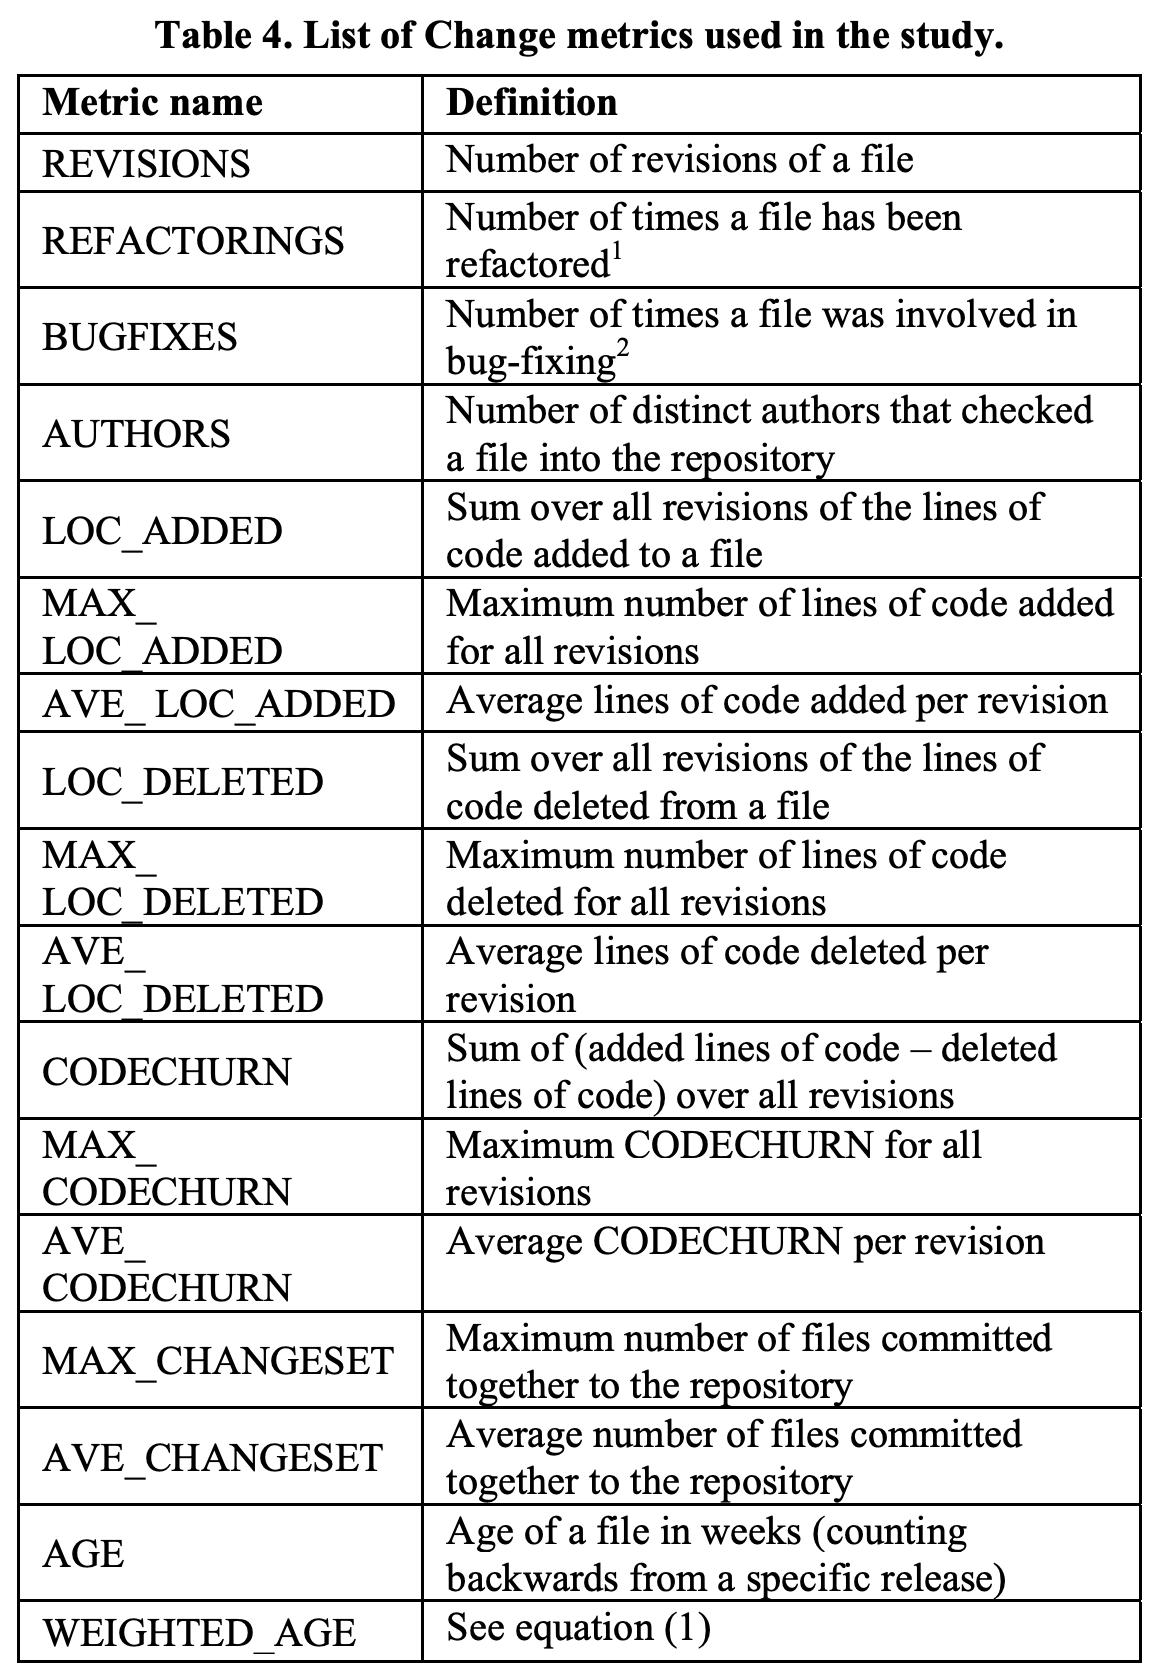
\includegraphics[width=.7\linewidth]{change-metrics.png}
\par\columnbreak\par
``Our set of change metrics is obviously only one possible proposal for change metrics we can extract from a CVS repository.''
\source{moser2008comparative}
\end{multicols}}

\qte
  [Abdulkareem Alali]
  {abdulkareem-alali.jpg}
  {One observation is that the terms that suggest \ul{bug related changes} are associated with fairly small-sized commits.}
  {alali2008s}

\pitch{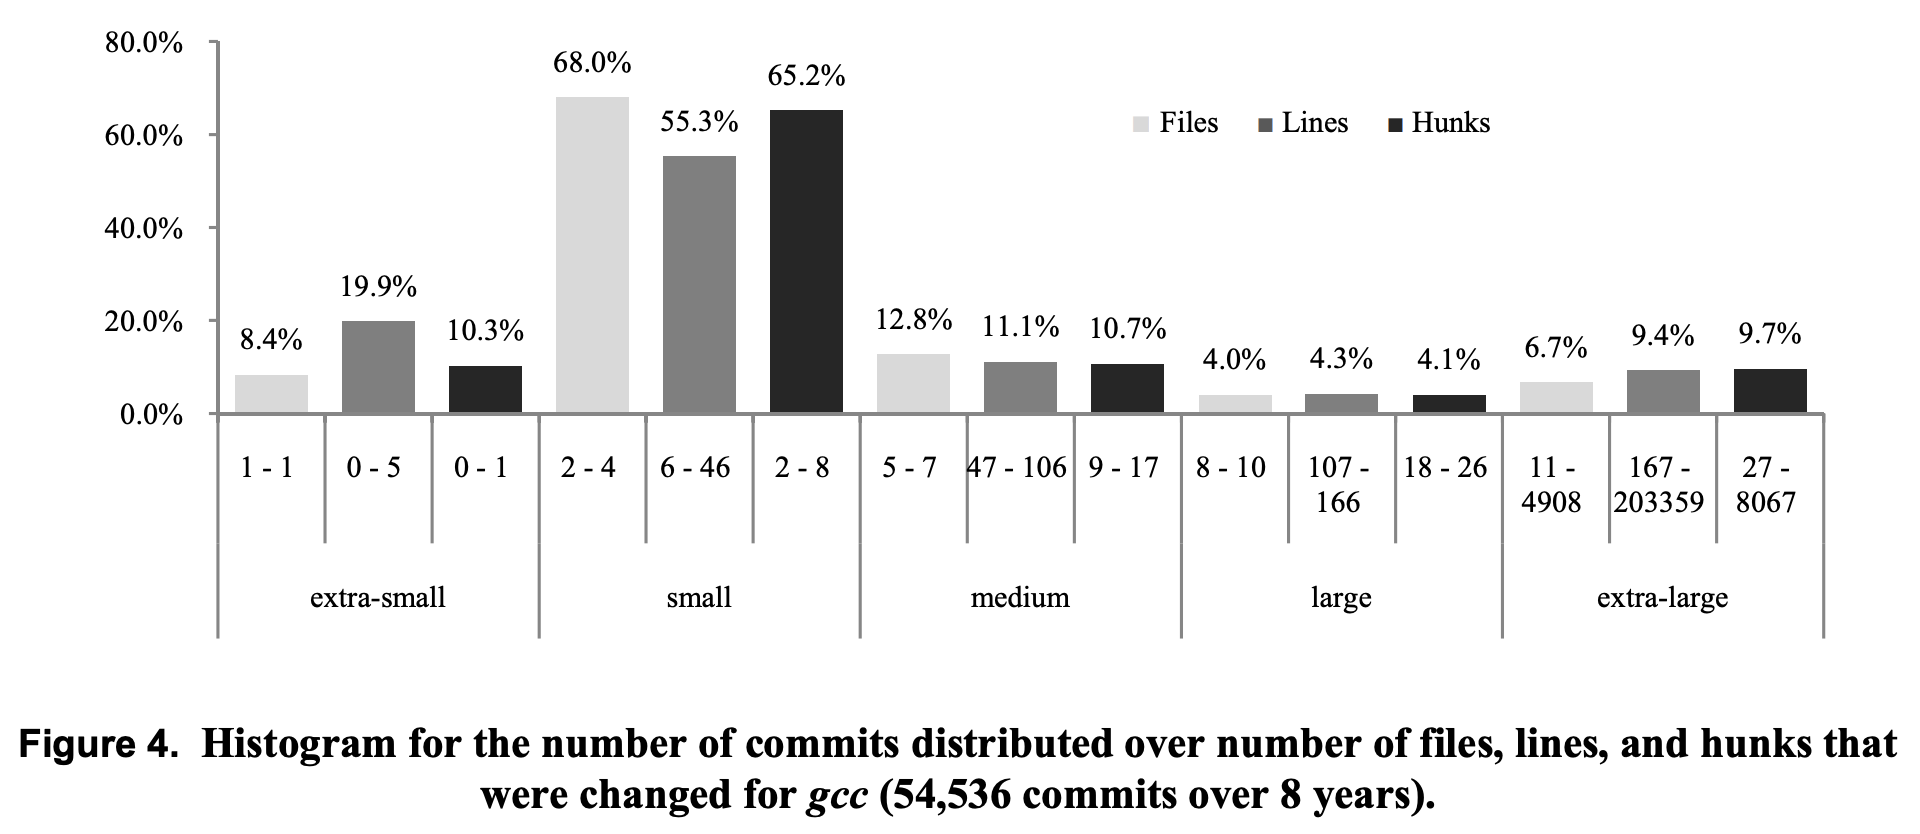
\includegraphics[width=.95\linewidth]{size-distribution.png}
\source{alali2008s}}

\pitch{\begin{multicols}{2}
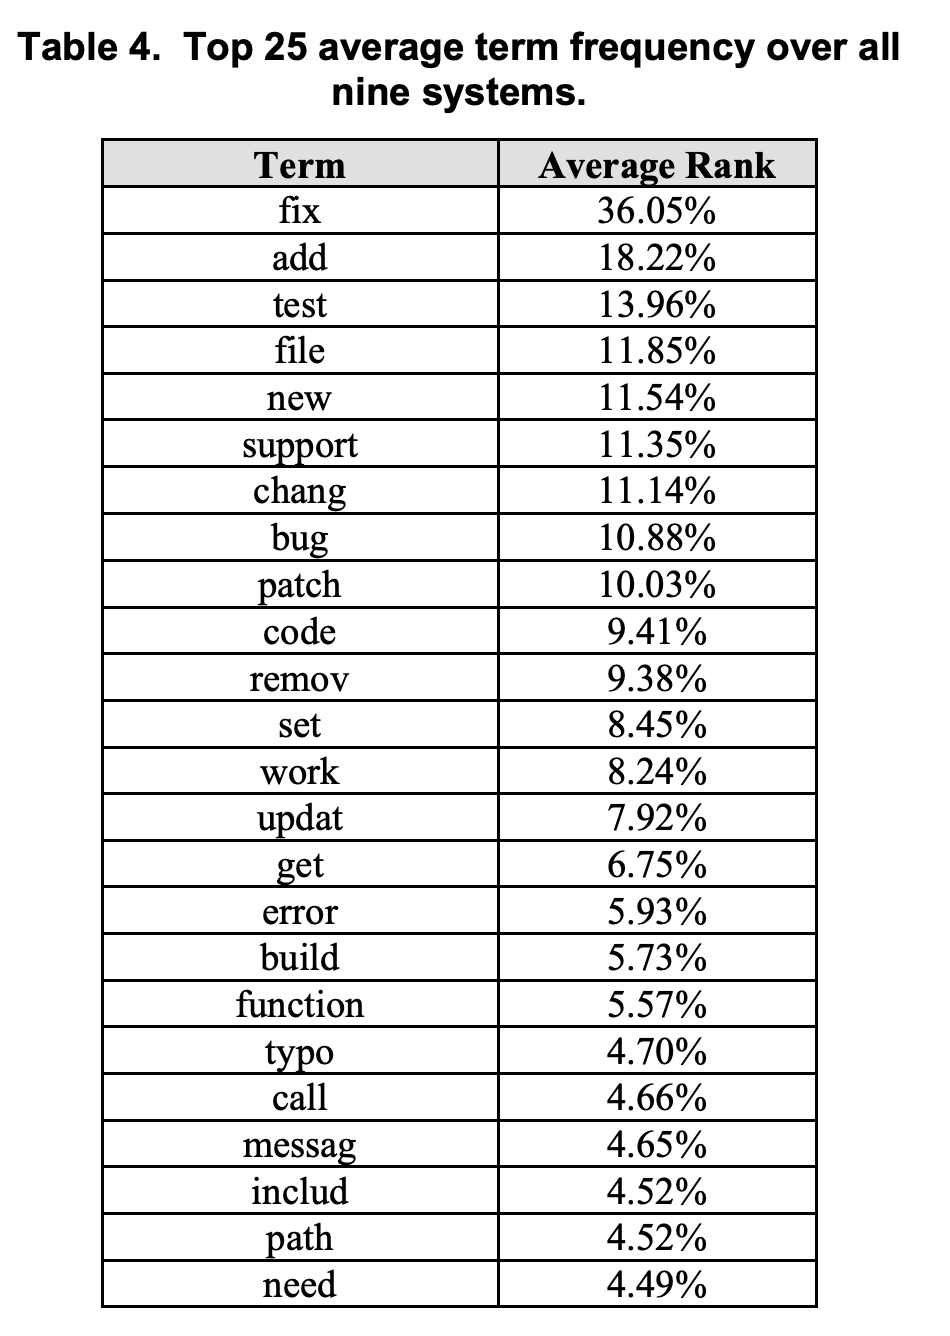
\includegraphics[width=.7\linewidth]{terms.png}
\par\columnbreak\par
``For each project, we collected the log messages and eliminated stop words using the \nospell{Lovins stemmer} algorithm... The result is a ranked list of frequent terms for each project. Then we cross join those nine lists and take the top most 50 frequent terms.''
\source{alali2008s}
\end{multicols}}

\qte
  [Abram Hindle]
  {abram-hindle.jpg}
  {Large commits were more likely to \ul{perfective} than \ul{corrective}, while small changes were more often corrective rather than perfective. In a way it makes sense, correcting errors is surgical, perfecting a system is much more global in scope.}
  {hindle2008large}

\pitch{\begin{multicols}{2}
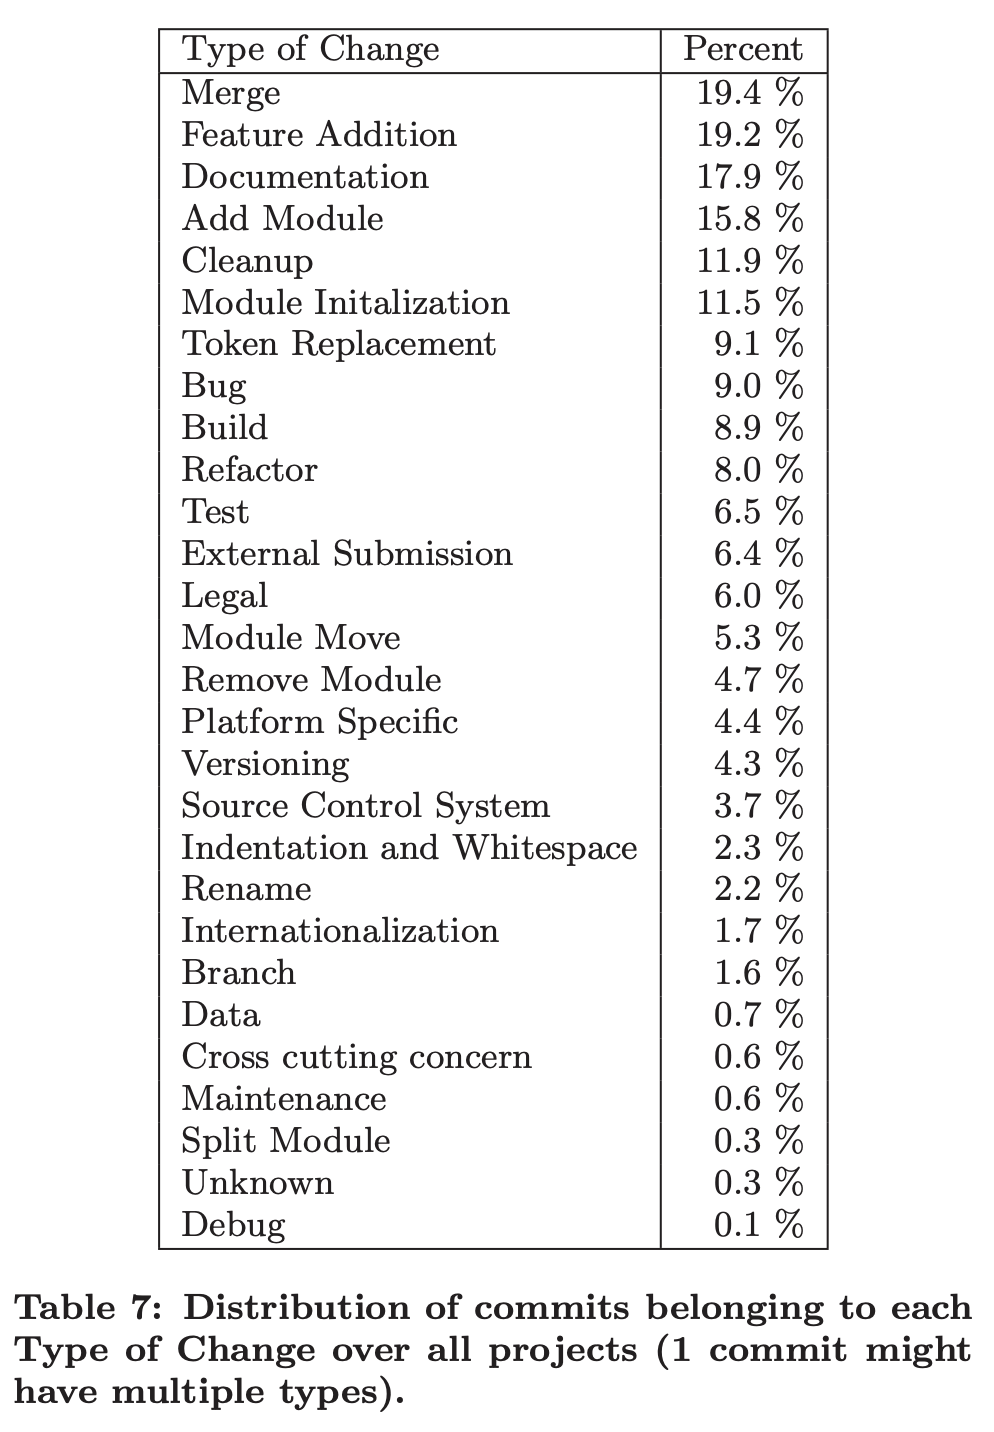
\includegraphics[width=.7\linewidth]{type-of-change.png}
\par\columnbreak\par
``We believe that reading a commit log and its diff gives an idea of how easy or difficult it is to maintain a system. For example, several features in PostgreSQL required large commits to be implemented. This is very \ul{subjective}, but reliable methods could be researched and developed to \ul{quantify} such effect.''
\source{hindle2008large}
\end{multicols}}

\qte
  [Oliver Arafat]
  {../19-comments-density/oliver-arafat.jpg}
  {We suggest distinguishing commit types by their size, using the following simple heuristic: \ul{single} commits of 1 to 100 SLoC, \ul{aggregate} commits of 101 to 10000 SLoC, and repository \ul{refactorings} of more than 10000 SLoC.}
  {arafat2009commit}

\qte
  [Marco D'Ambros]
  {marco-dambros.jpg}
  {Developers do not always document all the changes in the commit comment. A common cause is that writing exhaustive comments is \ul{time consuming}, and---being the last step of a coding session---the necessary \ul{time} and \ul{energy} is not always available. Moreover, for commits with many changes, the developers might \ul{not remember} all of the modifications.}
  {d2010commit}

\qte
  [Raymond Buse]
  {raymond-buse.jpg}
  {We present an automatic technique for synthesizing succinct human-readable documentation for arbitrary program \ul{differences}. We compare our documentation to 250 human-written log messages from 5 popular open source projects. Employing a human study, we find that our generated documentation is \ul{suitable} for supplementing or replacing 89\% of existing log messages that directly describe a code change.}
  {buse2010automatically}

\qte
  [Jon Eyolfson]
  {jon-eyolfson.jpg}
  {Commits submitted between midnight and 4~AM (referred to as late-night commits) are significantly buggier and commits between 7~AM and noon are less buggy, implying that developers may want to double-check their own latenight commits.}
  {eyolfson2011time}

\qte
  [Robert Dyer]
  {robert-dyer.jpg}
  {First, around 14\% of all log messages were completely \ul{empty}. Second, over two thirds of the messages contained \ul{1–15 words}, which is less than the average length of a sentence in English. A \ul{normal} length sentence in English is \ul{15–20 words} (according to various results in Google) and thus we see that very few logs (10\%) contained descriptive messages.}
  {dyer2013boa}

\qte
  [Luis Fernando Cort{\'e}s-Coy]
  {luis-fernando-cortes-coy.jpg}
  {The results of the user study demonstrate that 84\% of the \ul{generated} commit messages do not miss essential information required to understand the changes, 25\% of them are concise, and in 39\% of the cases the generated messages are easy to read and understand.}
  {cortes2014automatically}

\qte
  [Shane McIntosh]
  {shane-mcintosh.jpg}
  {JIT models, which aim to \ul{predict} the commits that will introduce \ul{future defects}, are typically trained using code-based metrics. We add metrics that estimate the level of detail in commit messages to JIT models with code-based metrics. We find that 43\% and 80\% of the JIT models of the studied systems are significantly improved by adding metrics that measure commit message \ul{volume} and \ul{content}, respectively.}
  {barnett2016relationship}

\qte
  [Jeongju Sohn]
  {jeongju-sohn.jpg}
  {\ul{Age} simply measures how long a given program element has existed in the code base. We calculate the age of a given \ul{statement} as the number of consecutive versions from the faulty version backwards to the latest version containing a modication to the statement.}
  {sohn2017fluccs}

\qte
  [Iftekhar Ahmed]
  {iftekhar-ahmed.jpg}
  {Commit message quality has an impact on software defect proneness, and the overall quality of the commit messages decreases over time, while developers believe they are writing better commit messages.}
  {li2023commit}

\qte
  [Yuxia Zhang]
  {yuxia-zhang.jpg}
  {Although LLMs can take larger diffs as input, their performance of generating messages leaves much to be improved. UniXcoder tends to generate short messages, while ChatGPT can generate more detailed messages, which are \ul{very different} from those written by developers.}
  {zhang2024automatic}

\plush{\pptBanner{Pitfalls of Automated Commits Generation}
\begin{pptWide}{2}{\small\begin{itemize}
\item ``Developers indicate that writing the subject of a commit message is \ul{hard}, and approximately 37\% of developers also find writing subjects \ul{time-consuming}.''
\item ``The state-of-the-art approaches for automated commit message generation have limited their datasets to commits whose diffs have \ul{no more than 100 or 200 tokens}. However, only 5\% of commits have a diff length of no more than 100 tokens. The performance of four state-of-the-art approaches on commits with larger diffs degrades significantly.''
\item ``After removing \ul{bot-generated} and \ul{uninformative} commit messages from the training and testing datasets, the performance of \nospell{NNGen}, \nospell{CoRec}, and \nospell{CCRep} greatly declines in comparison to the original evaluations.''
\end{itemize}}\end{pptWide}\source{zhang2024automatic}}

\plush{\pptBanner{Commits Best Practices (Coders' Folklore)}
\begin{multicols}{2}{\small\begin{itemize}
\item ``Commit it as soon as it compiles''
  --- \href{https://softwareengineering.stackexchange.com/a/74789/20873}{here}
\item ``Prefer small commits to large commits.''
  --- \href{https://softwareengineering.stackexchange.com/a/207036/20873}{here}
\item ``You shouldn't commit based on a time basis, but on a feature basis''
  --- \href{https://softwareengineering.stackexchange.com/a/74893/20873}{here}
\item ``I tend to commit anytime I take a break''
  --- \href{https://softwareengineering.stackexchange.com/a/74767/20873}{here}
\item ``If you have to put the word "and" or "also" in your summary, you need to split it up.''
  --- \href{https://softwareengineering.stackexchange.com/a/12209/20873}{here}
\item ``If you can't adequately comment a commit in one line, then it's already too large.''
  --- \href{https://softwareengineering.stackexchange.com/a/10944/20873}{here}
\end{itemize}}\end{multicols}}


\end{document}
